
%-------------------------------------------------------------------------------
%                             ADDITIONAL PACKAGES
%-------------------------------------------------------------------------------
\documentclass[
	a4paper,
%	showframes,
%	vline=2.2em,
%	maincolor=cvgreen,
%	sectioncolor=red,
%	subsectioncolor=orange,
%	itemtextcolor=black!80,
%	sidebarwidth=0.4\paperwidth,
%	topbottommargin=0.03\paperheight,
%	leftrightmargin=20pt,
%	profilepicsize=4.5cm,
%	profilepicborderwidth=3.5pt,
%	profilepicstyle=profilecircle,
%	profilepiczoom=1.0,
%	profilepicxshift=0mm,
%	profilepicyshift=0mm,
% profilepicrounding=1.0cm,
]{fortysecondscv}

% define divider and cvdivider command: dashed gray line separator
% attention: import colortbl befor arydshln
\usepackage{colortbl}
\usepackage{arydshln}
\RequirePackage{dashrule}
\colorlet{body}{black!80!white}
\newcommand{\cvdivider}{\arrayrulecolor{body!30}\hdashline}
\newcommand{\profiledivider}{\textcolor{body!30}{\hdashrule{\linewidth}{0.6pt}{0.5ex}}\\}
%\newcommand{\divider}{\textcolor{body!30}{\hdashrule{\linewidth}{0.6pt}{0.5ex}}}

% Portuguese package (used in signature date)
%\usepackage[portuguese]{babel}

% package used to wrap text around a figure
\usepackage{wrapfig}

% provides blind text useful for test purposes
\usepackage{blindtext}

\usepackage{amsmath}
\usepackage{makecell}

% table related packages
\usepackage{multirow}
\usepackage{array}
\newcolumntype{L}[1]{>{\raggedright\let\newline\\\arraybackslash\hspace{0pt}}m{#1}}
\newcolumntype{C}[1]{>{\centering\let\newline\\\arraybackslash\hspace{0pt}}m{#1}}
\newcolumntype{R}[1]{>{\raggedleft\let\newline\\\arraybackslash\hspace{0pt}}m{#1}}

% floating objects (figures, tables)
\usepackage{float}
% set font to any desired size
%\usepackage{anyfontsize}
% add font sizes \HUGE and \ssmall
%\usepackage[11pt]{moresize}

% multiple columns
\usepackage{multicol}
\usepackage{vwcol}

% adjust list spacing
\usepackage{enumitem}

% include fonts
\pdfmapfile{=ClearSans.map}
\pdfmapfile{=fontawesome.map}

% include and use scalable cm-super fonts
\usepackage[T1]{fontenc}
\usepackage{lmodern}

% improve word spacing and hyphenation
\usepackage{microtype}
\usepackage{ragged2e}

% provides blind text useful for test purposes
\usepackage{blindtext}

\usepackage{amsmath}

% include fonts
\pdfmapfile{=ClearSans.map}
\pdfmapfile{=fontawesome.map}

% include and use scalable cm-super fonts
\usepackage[T1]{fontenc}
\usepackage{lmodern}

% improve word spacing and hyphenation
\usepackage{microtype}
\usepackage{ragged2e}

% take care of proper font encoding
\ifxetexorluatex
	\usepackage{fontspec}
	\defaultfontfeatures{Ligatures=TeX}
%	\newfontfamily\headingfont[Path = fonts/]{segoeuib.ttf} % local font
\else
	\usepackage[utf8]{inputenc}
	\usepackage[T1]{fontenc}
%	\usepackage[sfdefault]{noto} % use noto google font
\fi

% enable mathematical syntax for some symbols like \varnothing
\usepackage{amssymb}

% bubble diagram configuration
%\usepackage{smartdiagram}
%\smartdiagramset{
%	% default font size is \large, so adjust to harmonize with sidebar layout
%	bubble center node font = \footnotesize,
%	bubble node font = \footnotesize,
%	% default: 4cm/2.5cm; make minimum diameter relative to sidebar size
%	bubble center node size = 0.4\sidebartextwidth,
%	bubble node size = 0.25\sidebartextwidth,
%	distance center/other bubbles = 1.5em,
%	% set center bubble color
%	bubble center node color = maincolor!70,
%	% define the list of colors usable in the diagram
%	set color list = {maincolor!10, maincolor!40,
%	maincolor!20, maincolor!60, maincolor!35},
%	% sets the opacity at which the bubbles are shown
%	bubble fill opacity = 0.8,
%}


%-------------------------------------------------------------------------------
%                            PERSONAL INFORMATION
%-------------------------------------------------------------------------------
%% mandatory information
% your name
\cvname{Rafael Claro Ito}
% job title/career
\cvjobtitle{
    Electrical Engineer\\[0.2em]
    HW \& SW Developer\\[0.2em]
    Data Scientist
}




%\graphicspath{{../figures/whoami/}}
%\newcommand{\whoamiemail}{\cvicon{\includegraphics[align=c, width=1.0em]{email}}}
%\whoamiemail




%% optional information
% profile picture
\cvprofilepic{../figures/profile.jpeg}

% NOTE: ordering in sidebar will mimic the following order
% date of birth
\cvbirthday{03/02/1992}
% short address/location, use \newline if more than 1 line is required
%\cvaddressone{Rua Gilberto Pattaro, 150 $\cdot$ Campinas/SP, Brazil}
\cvaddressone{Rua Gilberto Pattaro, 150 $\boldsymbol{\cdot}$ 13084-375}
\cvaddresstwo{Campinas, SP $\boldsymbol{\cdot}$ Brazil}
% phone number
\cvphone{+55 19 98810-2615}
% personal website
%\cvsite{https://pandascience.net}
% email address
\cvmail{ito.rafael@gmail.com}
% pgp key
%\cvkey{4096R/FF00FF00}{0xAABBCCDDFF00FF00}
% any other custom entry
%\cvcustomdata{\faFlag}{Chinese}

%\cvline{\hline}
%\cvline{}

\cvlinkedin{https://www.linkedin.com/in/itorafael/}{linkedin.com/in/itorafael}
\cvgithub{https://github.com/ito-rafael/}{github.com/ito-rafael}
\cvfacebook{https://www.facebook.com/ito.rafael92}{facebook.com/ito.rafael92}
\cvskype{}{ito.rafael92}
%\cvdocker{}{hub.docker.com/u/itorafael}
%\graphicspath{{../figures/}}
%\includegraphics[height=1em]{docker}
%hub.docker.com/u/itorafael

%-------------------------------------------------------------------------------
%                              SIDEBAR 1st PAGE
%-------------------------------------------------------------------------------
% add more profile sections to sidebar on first page
\addtofrontsidebar{

%    %===============
%    % SOCIAL NETWORK
%    %===============
%	% social network accounts incl. proper hyperlinks
%	\profilesection{Social Network}
%		\begin{icontable}{2.5em}{1em}
%%			\social{\aiOverleafSquare}
%				%{https://de.overleaf.com/latex/templates/forty-seconds-cv/pztcktmyngsk}
%			\social{\faLinkedin}
%                {https://www.linkedin.com/in/itorafael/}
%                {linkedin.com/in/itorafael}
%				%{LinkedIn}
%			\social{\faGithub}
%				{https://github.com/ito-rafael/}
%				{github.com/ito-rafael}
%				%{ito-rafael}
%            \social{\faFacebookSquare}
%                {https://www.facebook.com/ito.rafael92}
%                {facebook.com/ito.rafael92}
%            \social{\faSkype}
%                {}
%                {ito.rafael92}
%		\end{icontable}

    %===============
    % LANGUAGES
    %===============
	% include gosquare national flags from https://github.com/gosquared/flags;
	% naming according to ISO 3166-1 alpha-2 country codes
    \graphicspath{{../figures/languages/}}
	\profilesection{Languages}
		\pointskill{\flag{en-US}}{English}{5}
		\pointskill{\flag{pt-BR}}{Portuguese}{5}
	    \pointskill{\flag{it-IT}}{Italian}{4}
    	\pointskill{\flag{fr-FR}}{French}{2}
    	\pointskill{\flag{es-ES}}{Spanish}{2}
    	\pointskill{\flag{jp-JP}}{Japanese}{1}

    %===============
    % AWARDS
    %===============
    \profilesection{Awards}
        % insert path for awards icon
        \graphicspath{{../figures/awards/}}
        % define new commands for awars icon
        \newcommand{\goldenmedal}{\cvicon{
\includegraphics[align=c, width=1.0em]{medal_golden_red}}}
        \newcommand{\silvermedal}{\cvicon{
\includegraphics[align=c, width=1.0em]{medal_silver_blue}}}
        \newcommand{\certificate}{\cvicon{
\includegraphics[align=c, width=1.0em]{merit}}}
        \newcommand{\certificatetwo}{\cvicon{
\includegraphics[align=c, width=1.0em]{merit_2}}}
        
        \skill{\goldenmedal}{2009 6th place at OSA}
		\skill{\silvermedal}{2009 Silver Medal at OBMEP}
		\skill{\silvermedal}{2008 Silver Medal at OBMEP}
		\skill{\certificatetwo}{2008 Certificate of Merit at OMU}
		\skill{\certificate}{2007 Honorable Mention at OBMEP}
		\skill{\certificate}{2006 Honorable Mention at OBMEP}
        %--------------------------------------------------------
        \profiledivider
        {\scriptsize
            OBMEP: Brazilian Public Schools Mathematics Olympiad\\
            OSA: UNICAMP Physics Olympiad\\
            OMU: UNICAMP Mathematics Olympiad
            \par
        }

%	\profilesection{Hard Skills}
%		\skill{\faBalanceScale}{Sleeping almost all day}
%		\skill{\faSitemap}{Eating a lot bamboo sprouts}
%		\skill{\faGraduationCap}{Relaxing rest of the day}

%	\profilesection{Soft Skills}
%		\pointskill{\faHome}{Looking Cute}{4}[4]
%			\skill[1.8em]{\faCompress}{No need to specify further}
%		\pointskill{\faChild}{Chillin' hard}{3}[4]
%			\skill[1.8em]{\faCompress}{On a tree}
%			\skill[1.8em]{\faCompress}{On the grass}

}

%-------------------------------------------------------------------------------
%                              SIDEBAR 2nd PAGE
%-------------------------------------------------------------------------------
\addtobacksidebar{

%\normalsize
\small

    %===============
    % Coding Skils
    %===============
    \graphicspath{{../figures/coding/}}
    \profilesection{\LARGE{Programming Skills}}
        \pointskill{}{Python}{4}
        \hspace{6mm} \pointskill{\hspace{4mm} $\hookrightarrow$ \hspace{2mm}}{PyTorch}{4}
        \hspace{6mm} \pointskill{\hspace{4mm} $\hookrightarrow$ \hspace{2mm}}{NumPy}{4}
        \hspace{6mm} \pointskill{\hspace{4mm} $\hookrightarrow$ \hspace{2mm}}{Keras/TensorFlow}{2}
        \hspace{6mm} \pointskill{\hspace{4mm} $\hookrightarrow$ \hspace{2mm}}{scikit-learn}{4}
        \hspace{6mm} \pointskill{\hspace{4mm} $\hookrightarrow$ \hspace{2mm}}{skorch}{2}
        \hspace{6mm} \pointskill{\hspace{4mm} $\hookrightarrow$ \hspace{2mm}}{PyTorch Lightning}{3}
	\pointskill{}{C/C++}{3}
    \pointskill{}{Assembly}{3}
	\pointskill{}{VHDL}{1}
	\pointskill{}{Ladder Logic}{1}
	\pointskill{}{\LaTeX}{4}
    \vspace{-2mm}

    %===============
    % Softwares
    %===============
    \profilesection{\LARGE{Softwares Experiences}}
    \vspace{-3mm}
    \begin{itemize}
        \setlength\itemsep{0.0em}
        \item GNU/Linux
        \item MATLAB/Octave
        \item Git
        \item Docker
        \item Vagrant
        \item Jupyter Notebooks
        \item Anaconda
        \item Ansible
        \item Zabbix
        \item Qt
        \item CodeWarrior
        \item Kinetis Design Studio
        \item Quartus (Altera)
        \item AutoCAD
    \end{itemize}
    \vspace{-5mm}

    %===============
    % Embedded Systems
    %===============
    \profilesection{\LARGE{Embedded Systems}}
    \vspace{-3mm}
    \begin{itemize}
        \setlength\itemsep{0.0em}
        \item BeagleBone Black
        \item Raspberry Pi
        \item FRDM-KL25Z
        \item FRDM-K64F
        \item Arduino
        \item 8051
        \item PIC
        \item FPGA / CPLD
    \end{itemize}
    \vspace{-5mm}

    %===============
    % References
    %===============
    \profilesection{\LARGE{References}}
    	\cvreference
            {\textcolor{iconcolor}{\hskip 0.19em \large\faBriefcase} \hskip 0.1em
            \textbf{Fulano da Silva}
            \smallskip\newline\medskip
            Head of ...\newline
            $\boldsymbol{\cdot}$ \textbf{Relationship:} ex-boss\newline
            $\boldsymbol{\cdot}$ \textbf{Contact:} \href{mailto:fulanodasilva@gmail.com}{fulanodasilva@gmail.com}}
        %---------------------------------------
        \profiledivider
        %---------------------------------------
    	\cvreference
            {\vskip 0.7ex \textcolor{iconcolor}{\hskip 0.19em \large\faGraduationCap} \hskip 0.1em
            \textbf{Beltrano Souza}
            \smallskip\newline\medskip
            Professor at ...\newline
            $\boldsymbol{\cdot}$ \textbf{Relationship:} ex-professor\newline
        $\boldsymbol{\cdot}$ \textbf{Contact:} \href{mailto:beltrano@outlook.com}{beltrano@outlook.com}}
        %---------------------------------------

}

%	\profilesection{About Me}
%	\aboutme{
%		The giant panda is a terrestrial animal and primarily spends its life
%		roaming and feeding in the bamboo forests of the Qinling Mountains and in
%		the hilly province of Sichuan.
%	}
%
%	\profilesection{Diagrams}
%	\chartlabel{Bubble Diagram}
%	\begin{figure}\centering
%		\smartdiagram[bubble diagram]{
%			\textcolor{white}{\textbf{Being a}} \\
%			\textcolor{white}{\textbf{Panda}}, % center bubble
%			\textcolor{black!90}{Eating},
%			\textcolor{black!90}{Sleeping},
%			\textcolor{black!90}{Rolling},
%			\textcolor{black!90}{Playing},
%			\textcolor{black!90}{Chilling}
%		}
%	\end{figure}
%
%	\chartlabel{Wheel Chart}
%
%	\wheelchart{4em}{2em}{%
%	20/3em/maincolor!50/Chill,
%	15/3em/maincolor!15/Play,
%	30/4em/maincolor!40/Sleep,
%	20/3em/maincolor!20/Eat
%	}
%
%	\profilesection{Barskills}
%	\barskill{\faSkyatlas}{Wearing asian rice hats}{60}
%	\barskill{\faImage}{Playing Chess}{30}
%	\barskill{\faMusic}{Playing the bamboo flute}{50}
%
%	\profilesection{Memberships}
%	\begin{memberships}
%        \membership[4em]{../figures/logo.png}{PandaScience.net}
%        \membership[4em]{../figures/logo.png}{Some long text spanning over more than
%			only one line}
%            \membership[4em]{../figures/logo.png}{\rule{\linewidth}{1pt}}
%	\end{memberships}

%===============================================================================
%                         TABLE ENTRIES 1st PAGE
%===============================================================================
\begin{document}
\makefrontsidebar

%=======================================
\cvsection{Education}
%=======================================
%\cvsubsection{Postgraduate Training}
\graphicspath{{../figures/education/}}
%\begin{cvtable}[1.5]
    \cvevent
        {Graduate}
        {University of Campinas}
        {Jan 2017 -- current}
        {Campinas/SP}
        {\hspace{2mm}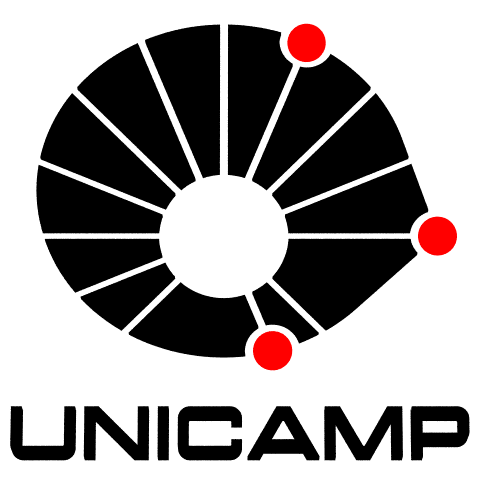
\includegraphics[height=0.07\textwidth]{Unicamp}}
        {Part-time Masters degree without being officially enrolled.
        %-------------------
        % set row color
        \newcommand{\rowgray}{\rowcolor[gray]{.95}}
        % set column separator
        \setlength{\tabcolsep}{3pt}
        %-------------------
        \begin{table}[H]
            \tiny
            \begin{center}
                \begin{tabular}{ |C{6.5mm}|m{6cm}|C{6mm}|m{2.6cm}|C{7.5mm}|C{9mm}| } 
                %              { |    subject    | cred |  prof  | semest | grade| } 
                    %=======================================
                    \hline
                    \rowcolor[gray]{0.75}
                    \multicolumn{2}{|c|}{Subject} & Credits & \multicolumn{1}{c|}{Professor(s)} & Semester & Grade \\
                    %=======================================
                    \hline
                    %-------------------
                    IA353A                                      &
                    Redes Neurais                               & 
                    4                                           & 
                    Fernando José Von Zuben                     &
                    1s2020                                      &
                    in progress                                 \\
                    %=======================================
                    \hline
                    \rowgray
                    & Tópicos Em Engenharia de Computação VII &&&&\\ 
                    %-------------------
                    \rowgray
                    \multirow{-2}{*}{IA376E}                    &
                    \hspace{1mm} $\hookrightarrow$ Redes Neurais Profundas Para Processamento de Linguagem Natural &
                    \multirow{-2}{*}{4}                         & 
                    \multirow{-2}{*}{Roberto de Alencar Lotufo} & 
                    \multirow{-2}{*}{1s2020}                    & 
                    \multirow{-2}{*}{in progress}               \\
                    %=======================================
                    \hline
                    %-------------------
                    \multirow{2}{*}{IA006C}                     & 
                    Tópicos em Sistemas Inteligentes II         & 
                    \multirow{2}{*}{4}                          & 
                    Levy Boccato                                & 
                    \multirow{2}{*}{2s2019}                     & 
                    \multirow{2}{*}{A}                          \\
                    %-------------------
                    & \hspace{1mm} $\hookrightarrow$ Aprendizado de Máquina && Romis Ribeiro de Faissol Attux &&\\
                    %=======================================
                    \hline
                    \rowgray
                    & Tópicos em Engenharia de Computação V     &&
                    Eleri Cardozo                               &&\\ 
                    %-------------------
                    \rowgray
                    \multirow{-2}{*}{IA368N}                    &
                    \hspace{1mm} $\hookrightarrow$ Introdução à Robótica Móvel &
                    \multirow{-2}{*}{4}                         & 
                    Eric Rohmer                                 &
                    \multirow{-2}{*}{2s2017}                    & 
                    \multirow{-2}{*}{A}                         \\
                    %=======================================
                    \hline
                    %-------------------
                    IA750A                                      & 
                    Engenharia de Reabilitação                  & 
                    4                                           & 
                    Antonio Augusto Fasolo Quevedo              & 
                    2s2017                                      & 
                    A                                           \\
                    %=======================================
                    \hline
                    \rowgray
                    & Tópicos em Engenharia de Computação V     &&
                    Eleri Cardozo                               &&\\ 
                    %-------------------
                    \rowgray
                    \multirow{-2}{*}{IA368W}                    & 
                    \hspace{1mm} $\hookrightarrow$ Métodos Estocásticos Para Robótica Móvel &
                    \multirow{-2}{*}{4}                         &
                    Eric Rohmer                                 &
                    \multirow{-2}{*}{1s2017}                    & 
                    \multirow{-2}{*}{A}                         \\
                    %=======================================
                    \hline
                    %-------------------
                    \multirow{2}{*}{IE327P}                     & 
                    Tópicos Especiais em Microeletrônica III    & 
                    \multirow{2}{*}{4}                          & 
                    \multirow{2}{*}{Elnatan Chagas Ferreira}    & 
                    \multirow{2}{*}{1s2017}                     & 
                    \multirow{2}{*}{A}                          \\
                    %-------------------
                    & \hspace{1mm} $\hookrightarrow$ Sensores, Condicionamento e Aquisição de Dados &&&&\\
                    %=======================================
                    \hline
                    \multicolumn{6}{l}{ }\\
                    \multicolumn{6}{r}{* table information in Portuguese}
                    %=======================================
                \end{tabular}
            \end{center}
            %\caption{}
            %\label{tab:}
        \end{table}
        }
    \vspace{-8mm}

    %---------------------------------------
    \profiledivider
    %---------------------------------------
	\cvevent
        {Undergraduate}
        {University of Campinas}
        {Jan 2011 -- Dec 2016}
        {Campinas/SP}
        {\hspace{2mm}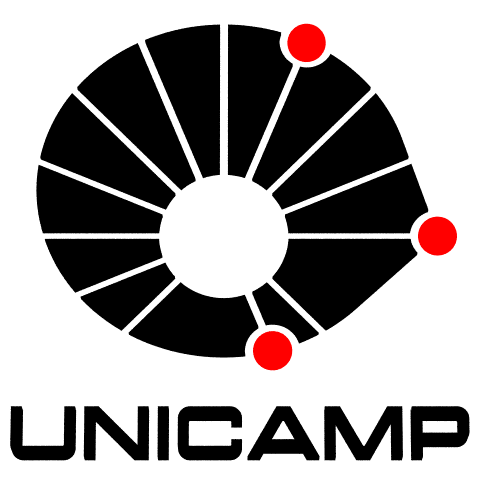
\includegraphics[height=0.07\textwidth]{Unicamp}}
        { 
        \vspace{-2mm}
        % set column separator
        \setlength{\tabcolsep}{3pt}
        \begin{table}[H]
            \tiny
            \begin{center}
                \begin{tabular}{ |C{6.5mm}|m{5.8cm}|C{6mm}|C{2.1cm}|C{17.5mm}|C{6mm}| }
                %              { |     subject     | cred |  prof  | semestr | grade| }
                    \hline
                    \rowcolor[gray]{0.75}
                    \multicolumn{2}{|c|}{Subject} & Credits & Professor & Semester & Grade \\
                    %=======================================
                    \hline
                    \multirow{2}{*}{EA999A}                     &
                    Tópicos em Egenharia de Computação          &
                    \multirow{2}{*}{4}                          &
                    \multirow{2}{*}{Roberto de Alencar Lotufo}  &
                    \multirow{2}{*}{Férias de Verão 2020}       &
                    \multirow{2}{*}{8.9}                        \\
                    %-------------------
                    & \hspace{1mm} $\hookrightarrow$ Curso Teórico-Prático de Redes Neurais Convolucionais &&&&\\
                    %=======================================
                    \hline
                    \multicolumn{6}{l}{ }\\
                    \multicolumn{6}{r}{* table information in Portuguese}
                    %=======================================
                 \end{tabular}
            \end{center}
            %\caption{}
            %\label{tab:}
        \end{table}
        }
    \vspace{-8mm}

    %---------------------------------------
    \profiledivider
    %---------------------------------------
    \cvevent
        {Undergraduate (Student Exchange Program)}
        {Queen Mary University of London}
        {Sep 2014 -- Aug 2015}
        {London}
        {\hspace{2mm}
\includegraphics[height=0.05\textwidth]{QMUL}}
        {Studies sponsored by the Brazilian government due to academic merit. Science without Borders (SwB) student exchange program.}

    %---------------------------------------
    \profiledivider
    %---------------------------------------
	\cvevent
        {Further Education}
        {Technical College of Campinas - UNICAMP}
        {Jan 2007 -- Jul 2010}
        {Campinas/SP}
        {\hspace{2mm}
\includegraphics[height=0.07\textwidth]{Cotuca}}
        {Selected to work as a Teaching Assistant of the technical course.}

%=======================================
\cvsection{\href{https://github.com/ito-rafael/machine-learning}{\faGithub}\hspace{0.5mm} Machine Learning Portfolio}
%=======================================
\vspace{3mm}
%-------------------
% change item symbols
\renewcommand{\labelitemi}{\textbullet}
\renewcommand{\labelitemii}{\textbullet}
\renewcommand{\labelitemiii}{\textbullet}
\renewcommand{\labelitemiv}{\textbullet}
%-------------------
% include images path
\graphicspath{{../figures/machine-learning-portfolio/}}
% GitHub icon
\newcommand{\github}[1]{\href{#1}{\faGithub}}
% Google Colab icon
\newcommand{\colab}[1]{\href{#1}{\includegraphics[height=1em]{colab}}}
%-------------------
%\begin{multicols}{2}
%\begin{vwcol}[widths={0.45,0.55}, sep=.8cm, justify=flush,rule=0pt,indent=1em]
\begin{minipage}[t]{0.45\linewidth}

\small
\textbf{\color{sectioncolor}Jupyter notebooks:}\\\\
\scriptsize
%---------------------------------------
\textbf{\underline{Computer Vision:}}
%---------------------------------------
\begin{itemize}[leftmargin=*,labelindent=3mm,labelsep=1mm]
    %---------------------------------------
    \item MNIST: Linear Classifier
        \hfill
        \github{https://github.com/ito-rafael/machine-learning/blob/master/notebooks/computer\%20vision/MNIST\%20-\%20Linear.ipynb}
        \hspace{0.1mm}
        \colab{https://colab.research.google.com/drive/1QTgLwLK3BEfQV0fi_HasQsL1Zm-6l4A4?usp=sharing}
    %---------------------------------------
    \item MNIST: Extreme Learning Machine (ELM)
        \hfill
        \github{https://github.com/ito-rafael/machine-learning/blob/master/notebooks/computer\%20vision/MNIST\%20-\%20ELM.ipynb}
        \hspace{0.1mm}
        \colab{https://colab.research.google.com/drive/1FUbVaGFz9UmNx9NP45wHZC0Of7WMz75r?usp=sharing}
    %---------------------------------------
    \item MNIST: Multilayer Perceptron (MLP)
        \hfill
        \github{https://github.com/ito-rafael/machine-learning/blob/master/notebooks/computer\%20vision/MNIST\%20-\%20MLP.ipynb}
        \hspace{0.1mm}
        \colab{https://colab.research.google.com/drive/1OKWU4uYmgj7YWWC8o2UKolOPtqimSBfK?usp=sharing}
    %---------------------------------------
    \item MNIST: ConvNet (CNN)
        \hfill
        \github{https://github.com/ito-rafael/machine-learning/blob/master/notebooks/computer\%20vision/MNIST\%20-\%20ConvNet.ipynb}
        \hspace{0.1mm}
        \colab{https://colab.research.google.com/drive/1Ne6y2G_rsH4bYoItFveRA29N0NZ9ZZL_?usp=sharing}
    %---------------------------------------
    \item Transfer Learning: Cats and Dogs
        \hfill
        \github{https://github.com/ito-rafael/machine-learning/blob/master/notebooks/computer\%20vision/Transfer\%20Learning\%20-\%20Cats\%20\%26\%20Dogs.ipynb}
        \hspace{0.1mm}
        \colab{https://colab.research.google.com/drive/1okJH91odJWQXn5pScQfVyjkAYTvH06Sk}
    %---------------------------------------
    \item Transfer Learning (last layer): Fruits360
        \hfill
        \github{https://github.com/ito-rafael/machine-learning/blob/master/notebooks/computer\%20vision/Transfer\%20Learning\%20-\%20Fruits360\%20(only\%20last\%20layer).ipynb}
        \hspace{0.1mm}
        \colab{https://colab.research.google.com/drive/18d_M9U0uxQ0lAOqoiHA18ekjQq4xNX4D}
    %---------------------------------------
    \item Transfer Learning (fine tuning): Fruits360
        \hfill
        \github{https://github.com/ito-rafael/machine-learning/blob/master/notebooks/computer\%20vision/Transfer\%20Learning\%20-\%20Fruits360\%20(fine-tunning).ipynb}
        \hspace{0.1mm}
        \colab{https://colab.research.google.com/drive/1R9xNZk7E1C-_5x_AW_r2PA5NDBrNqKEb}
    %---------------------------------------
\end{itemize}
\vspace{2mm}

%---------------------------------------
\textbf{\underline{Natural Language Processing (NLP):}}
%---------------------------------------
\begin{itemize}[leftmargin=*,labelindent=3mm,labelsep=1mm]
    %---------------------------------------
    \item Language Model
        \hfill
        \github{https://github.com/ito-rafael/IA376E-NLP_DeepLearning-1s2020/blob/master/Aula\%203/Language_Model_(Rafael_Ito).ipynb}
        \hspace{0.1mm}
        \colab{https://colab.research.google.com/drive/1bN7PZKTg5tNFbshVDpeDs2SyO0ry7t-g}
    %---------------------------------------
    \item Sentiment Analysis (IMDb dataset) using:
    \begin{itemize}[leftmargin=*,labelindent=2mm,labelsep=1mm]
        %-------------------
        \item Bag-of-Words
            \hfill
            \github{https://github.com/ito-rafael/IA376E-NLP_DeepLearning-1s2020/blob/master/Aula\%202/IMDb_Sentiment_analysis_(Rafael_Ito).ipynb}
            \hspace{0.1mm}
            \colab{https://colab.research.google.com/drive/1CTPhLShW60HhVE0zzQFTq45jRiEKPKcR}
        %-------------------
        \item TF-IDF
            \hfill
            \github{https://github.com/ito-rafael/IA376E-NLP_DeepLearning-1s2020/blob/master/Aula\%204/IMDb_Sentiment_analysis_with_(Rafael_Ito).ipynb}
            \hspace{0.1mm}
            \colab{https://colab.research.google.com/drive/1ynG17D67-hi78xPcEkHzxalsaMmut9z6}
        %-------------------
        \item Simplified Self-Attention
            \hfill
            \github{https://github.com/ito-rafael/IA376E-NLP_DeepLearning-1s2020/blob/master/Aula\%205/IMDb_Sentiment_analysis_(Self_Attention_simple)_(Rafael_Ito).ipynb}
            \hspace{0.1mm}
            \colab{https://colab.research.google.com/drive/1DZKqRb-wW8waV2z27KQFKQHD73p5QxIQ}
        %-------------------
        \item Transformer (Encoder only)
            \hfill
            \github{https://github.com/ito-rafael/IA376E-NLP_DeepLearning-1s2020/blob/master/Aula\%206/IMDb_Sentiment_analysis_(Self_Attention_complete)_(Rafael_Ito).ipynb}
            \hspace{0.1mm}
            \colab{https://colab.research.google.com/drive/1G1qezkPK8HNyX3JuaqthZYgLnvz_fDvY}
        %-------------------
        \item BERT
            \hfill
            \github{https://github.com/ito-rafael/IA376E-NLP_DeepLearning-1s2020/blob/master/Aula\%208/Aula_8_BERT_(Rafael_Ito).ipynb}
            \hspace{0.1mm}
            \colab{https://colab.research.google.com/drive/1N6cw_YLv9bBXqF82b4pM_KJ3ms_-4o5z?authuser=1}
        %-------------------
    \end{itemize}
    %---------------------------------------
    \item T5 English to Portuguese Translator
            \hfill
            \github{https://github.com/ito-rafael/IA376E-NLP_DeepLearning-1s2020/blob/master/Aula\%209/Aula_9_T5_(English_Portuguese_translation)_(Rafael_Ito).ipynb}
            \hspace{0.1mm}
            \colab{https://colab.research.google.com/drive/192AWnbDwBnVX0uKiDF7dRfYH-1MxAd15}
\end{itemize}
\vspace{2mm}

%---------------------------------------
\textbf{\underline{Video Processing:}}
%---------------------------------------
\begin{itemize}[leftmargin=*,labelindent=3mm,labelsep=1mm]
    %---------------------------------------
    \item YOLO
        \hfill
        in progress
%        \github{}
%        \hspace{0.1mm}
%        \colab{}
    %---------------------------------------
    \item MobileNets
        \hfill
        in progress
%        \github{}
%        \hspace{0.1mm}
%        \colab{}
    %---------------------------------------
\end{itemize}
%---------------------------------------

\end{minipage}
\hspace{1mm}
%=======================================
\begin{minipage}[t]{0.53\linewidth}
\small
\textbf{\color{sectioncolor}One-page papers summary:}
\vspace{3.0mm}\\
\scriptsize
%\tiny
* available only in Portuguese

%-------------------
% Google Drive icon
\newcommand{\drive}[1]{\href{#1}{\includegraphics[height=1em]{drive}}}
% PDF icon
\newcommand{\pdf}[1]{\href{#1}{\hspace{1mm}\includegraphics[height=1em]{pdf}\\}}
%-------------------
\begin{itemize}[leftmargin=*,labelindent=3mm,labelsep=1mm]
%    %---------------------------------------
%    \item "title", year
%    %---------------------------------------
%%        \hfill
%        \pdf{}
%        \hfill
%        \hspace{2mm} $\hookrightarrow$ summary: 
%            \github{}
%            \hspace{0.1mm}
%            \drive{}
    %---------------------------------------
    \item "A Neural Probabilistic Language Model", 2003
    %---------------------------------------
%        \hfill
        \pdf{http://www.jmlr.org/papers/volume3/bengio03a/bengio03a.pdf}
        \hfill
        \hspace{2mm} $\hookrightarrow$ summary: 
            \github{https://github.com/ito-rafael/machine-learning/blob/master/one-page\%20papers\%20summary/2003\%20-\%20\%5BLanguage\%20Model\%5D\%20A\%20Neural\%20Probabilistic\%20Language\%20Model\%20\%5BYoshua\%20Bengio\%20-\%20Universit\%C3\%A9\%20de\%20Montr\%C3\%A9al\%5D.pdf}
            \hspace{0.1mm}
            \drive{https://docs.google.com/document/d/1MBboy05JIT-TyNyTxl-ppMgO-4PvaaaZrnW-M1L-0yI/edit?usp=sharing}
    %---------------------------------------
    \item "A Unified Architecture for Natural Language Processing: Deep Neural Networks with Multitask Learning", 2008
    %---------------------------------------
%        \hfill
        \pdf{https://ronan.collobert.com/pub/matos/2008_nlp_icml.pdf}
        \hfill
        \hspace{2mm} $\hookrightarrow$ summary: 
            \github{https://github.com/ito-rafael/machine-learning/blob/master/one-page\%20papers\%20summary/2008\%20-\%20\%5BMultitask\%20NLP\%5D\%20A\%20Unified\%20Architecture\%20for\%20Natural\%20Language\%20Processing:\%20Deep\%20Neural\%20Networks\%20with\%20Multitask\%20Learning\%20\%5BRonan\%20Collobert\%2C\%20Jason\%20Weston\%5D.pdf} 
            \hspace{0.1mm}
        \drive{https://docs.google.com/document/d/1jd6sd-SxfUYHUdh8hbLCDcR_PZ11d51tiEEHWcL3-zE/edit?usp=sharing} 
    %---------------------------------------
    \item "Efficient Estimation of Word Representations in Vector Space", 2013
    %---------------------------------------
%        \hfill
        \pdf{https://arxiv.org/pdf/1301.3781.pdf}
        \hfill
        \hspace{2mm} $\hookrightarrow$ summary: 
            \github{https://github.com/ito-rafael/machine-learning/blob/master/one-page\%20papers\%20summary/2013\%20-\%20\%5Bword2vec\%5D\%20Efficient\%20Estimation\%20of\%20Word\%20Representations\%20in\%20Vector\%20Space\%20\%5BGoogle\%20Inc\%5D.pdf} 
            \hspace{0.1mm}
            \drive{https://docs.google.com/document/d/11MRzz4_oK4KjUcnqLXI2B7Z2WDYRz7PtxctMZcjm2GA/edit?usp=sharing} 
    %---------------------------------------
    \item "Empirical Evaluation of Gated Recurrent Neural Networks on Sequence Modeling", 2014
    %---------------------------------------
%        \hfill
        \pdf{https://arxiv.org/pdf/1412.3555.pdf}
        \hfill
        \hspace{2mm} $\hookrightarrow$ summary: 
            \github{https://github.com/ito-rafael/machine-learning/blob/master/one-page\%20papers\%20summary/2014\%20-\%20\%5BLSTM\%2C\%20GRU\%5D\%20Empirical\%20Evaluation\%20of\%20Gated\%20Recurrent\%20Neural\%20Networks\%20on\%20Sequence\%20Modeling\%20(Chung\%20et\%20al.\%2C\%202014)\%20\%5BUniversit\%C3\%A9\%20de\%20Montr\%C3\%A9al\%5D.pdf}
            \hspace{0.1mm}
            \drive{https://docs.google.com/document/d/1X-guAkdcDhx84mH1xbaTaTxpZnYvBVMFrADq2IlPKE4/edit?usp=sharing}
    %---------------------------------------
    \item "Deep Learning", 2015
    %---------------------------------------
 %       \hfill
        \pdf{https://s3.us-east-2.amazonaws.com/hkg-website-assets/static/pages/files/DeepLearning.pdf}
        \hfill
        \hspace{2mm} $\hookrightarrow$ summary: 
            \github{https://github.com/ito-rafael/machine-learning/blob/master/one-page\%20papers\%20summary/2015\%20-\%20\%5BDeep\%20Learning\%5D\%20Deep\%20Learning\%20\%5BYann\%20LeCun\%2C\%20Yoshua\%20Bengio\%2C\%20Geoffrey\%20Hinton\%5D.pdf}
            \hspace{0.1mm}
            \drive{https://docs.google.com/document/d/1RW47cxVSiQoWAZ74jlFNnT6s5Q_6Ey7ua_uIBcmNBeg/edit?usp=sharing}
    %---------------------------------------
    \item "Effective Approaches to Attention-based Neural Machine Translation", 2015
    %---------------------------------------
%        \hfill
        \pdf{https://arxiv.org/pdf/1508.04025.pdf}
        \hfill
        \hspace{2mm} $\hookrightarrow$ summary: 
            \github{https://github.com/ito-rafael/machine-learning/blob/master/one-page\%20papers\%20summary/2015\%20-\%20\%5BAttention\%20NMT\%5D\%20Effective\%20Approaches\%20to\%20Attention-based\%20Neural\%20Machine\%20Translation\%20\%5BStanford\%5D.pdf} 
            \hspace{0.1mm}
            \drive{https://docs.google.com/document/d/13iF8bPHbeW97mOck_Ncqxtt_U4vkHXtaPbkqE-sPcww/edit?usp=sharing} 
    %---------------------------------------
    \item "Attention Is All You Need", 2017
    %---------------------------------------
%        \hfill
        \pdf{https://arxiv.org/pdf/1706.03762.pdf}
        \hfill
        \hspace{2mm} $\hookrightarrow$ summary: 
            \github{https://github.com/ito-rafael/machine-learning/blob/master/one-page\%20papers\%20summary/2017\%20-\%20\%5BTransformer\%5D\%20Attention\%20Is\%20All\%20You\%20Need\%20\%5BGoogle\%20Brain\%5D\%20(Vaswani\%20et\%20al.\%2C\%202017).pdf} 
            \hspace{0.1mm}
            \drive{https://docs.google.com/document/d/1pCnipY7b_Qcs0w1HAw8W9jDGRrzmH1KixT9Rlg8Mu0E/edit?usp=sharing} 
    %---------------------------------------
    \item "BERT: Pre-training of Deep Bidirectional Transformers for Language Understanding", 2019
    %---------------------------------------
%        \hfill
        \pdf{https://arxiv.org/pdf/1810.04805.pdf}
        \hfill
        \hspace{2mm} $\hookrightarrow$ summary: 
            \github{https://github.com/ito-rafael/machine-learning/blob/master/one-page\%20papers\%20summary/2019\%20-\%20\%5BBERT\%5D\%20BERT:\%20Pre-training\%20of\%20Deep\%20Bidirectional\%20Transformers\%20for\%20Language\%20Understanding\%20\%5BGoogle\%20AI\%20Language\%5D\%20(Devlin\%20et\%20al.\%2C\%202019).pdf} 
            \hspace{0.1mm}
            \drive{https://docs.google.com/document/d/1Yrd7j6UAQkS0ZHbjl-893eqiQuCVXFj1b4tOv2QHb1w/edit?usp=sharing} 
    %---------------------------------------
    \item "Exploring the Limits of Transfer Learning with a Unified Text-to-Text Transformer", 2019
    %---------------------------------------
%        \hfill
        \pdf{https://arxiv.org/pdf/1910.10683.pdf}
        \hfill
        \hspace{2mm} $\hookrightarrow$ summary: 
            \github{https://github.com/ito-rafael/machine-learning/blob/master/one-page\%20papers\%20summary/2019\%20-\%20\%5BT5\%5D\%20Exploring\%20the\%20Limits\%20of\%20Transfer\%20Learning\%20with\%20a\%20Unified\%20Text-to-Text\%20Transformer\%20\%5BGoogle\%5D.pdf} 
            \hspace{0.1mm}
            \drive{https://docs.google.com/document/d/13HLEYCKsRb_EJRauQyZpAOuXUhTC4GrDlFDhW5l-A-o/edit?usp=sharing} 
    %---------------------------------------
    \item "The Curious Case of Neural Text Degeneration", 2019
    %---------------------------------------
%        \hfill
        \pdf{https://arxiv.org/pdf/1904.09751.pdf}
        \hfill
        \hspace{2mm} $\hookrightarrow$ summary: 
            \github{https://github.com/ito-rafael/machine-learning/blob/master/one-page\%20papers\%20summary/2019\%20-\%20\%5BNucleus\%20Sampling\%5D\%20The\%20Curious\%20Case\%20of\%20Neural\%20Text\%20Degeneration\%20\%5BAllen\%20Institute\%20for\%20Artificial\%20Intelligence\%5D.pdf} 
            \hspace{0.1mm}
            \drive{https://docs.google.com/document/d/1IcBG9UQJNIfzteAGzPU7q-_wfBZnGPQ4H5GUwI-Q7EQ/edit?usp=sharing} 
    %---------------------------------------

\end{itemize}

\end{minipage}
%\end{multicols}
%\end{vwcol}

%%=======================================
%\cvsection{Awards}
%%=======================================
%\begin{cvtable}
%	\cvitem{2010 -- now}{Panda of the Year}{Panda World Forum}{}
%	\cvitem{2005 -- now}{Face of World Wide Fund for Nature}{WWF}{}
%	\cvitem{2000}{Winner of Bamboo Sprouts Eating Contest}{Bamboo Society}{}
%\end{cvtable}
%
%
%%=======================================
%\cvsection{Extra-Curricular Activities}
%%=======================================
%\begin{cvtable}
%	\cvitemshort{Relaxing}{Master the fine art of relaxing everywhere}
%	\cvitemshort{Music}{Playing the bamboo flute in the 1st Panda Orchestra}
%	\cvitemshort{Education}{Teaching young pandas to be more panda-like}
%\end{cvtable}

%===============================================================================
%                         TABLE ENTRIES 2nd PAGE
%===============================================================================
\newpage
\makebacksidebar

%=======================================
\cvsection{Working Experience}
%=======================================
% change arraystretch (distance between items):
%\begin{cvtable}[<arraystretch>=1]
%\begin{cvtable}[1.5]
%-------------------
% include images path
\graphicspath{{../figures/work/}}
%-------------------
    \cvevent
        {Technological Development Analyst}
        {CNPEM/LNLS}
        {Jan 2016 -- current}
        {Campinas/SP}
        {\hspace{2mm}
\includegraphics[height=0.05\textwidth]{CNPEM}}
        {Undergraduate internship realized at LNLS (Brazilian Synchrotron Light Laboratory) during the year of 2016 at the Controls Group with focus in hardware and software projects for the Sirius particle accelerator. At this period, projects with microcontrollers, single board computers, and platforms like BeagleBone Black and Green, Kinetis development platform KL25Z and K64F, and CPLD projects were developed.\\
        At the beginning of 2017, I was hired as Technological Development Analyst. Most of the projects consisted of the development of hardware and software to remotely control devices. The controls system platform adopted is the EPICS. Network management, Linux servers maintenance and interns mentorship were also related activities.
        \begin{itemize}
            \item \github{https://github.com/lnls-sirius/spixconv} \hspace{0.5mm} \textbf{SPIxCONV:} This project consists of an 18-bit analog input (ADC) and output (DAC) within a range of 20 V ($\pm$ 10 V) and 32 digital pins that can be either as inputs or outputs. This system interfaces with pulsed power electronics hardware in order to control the output voltage for pulsed magnets as well as read and write status commands to their power supplies. An operator interface (OPI) software based on Qt was also developed for remote control.
            \item \github{https://github.com/lnls-sirius/vacuum-bbb-controller} \hspace{0.5mm} \textbf{VBC:} This project (vacuum-bbb-controller) consists of a hardware based on BeagleBone Black that controls (read and write) a pump station. Several devices are controlled, such as mechanical pump, turbomolecular pump and valves. An OPI for remote control was also developed.
            \item \github{https://github.com/lnls-sirius/pydm-opi} \hspace{0.5mm} \textbf{pydm-opi:} Set of all OPI screens built with PyDM (PyQt-based framework) developed by the Controls Group of LNLS.
            \item \github{https://github.com/lnls-sirius/mailpy} \hspace{0.5mm} \textbf{mailpy:} Python script that monitors several variables, check their specified operation values and send e-mails to a list of targets with a warning message if the variable value exceed its limits.
        \end{itemize}
        }
    %---------------------------------------
    \profiledivider
    %---------------------------------------
    \vspace{-2.2mm}
    \cvevent
        {Teaching Assistant}
        {University of Campinas}
        {Jan 2016 -- Jul 2016}
        {Campinas/SP}
        {\hspace{2mm}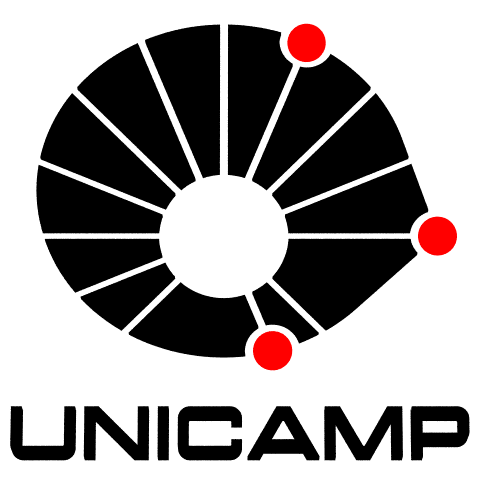
\includegraphics[height=0.07\textwidth]{Unicamp}}
        {During this period I was responsible for helping the teacher to prepare the laboratory experiments and to help the students with all the laboratory classes of the subject EE641 (Basic Electronics Lab II). Several projects for the platform Raspberry Pi were developed. For example, PWM controllers, wireless data transmission, temperature sensor with thermostat, R/2R ladder DAC, Successive approximation ADC, ECG waveform generator and signal recorder.}
    %---------------------------------------
    \\\profiledivider
    %---------------------------------------
    \vspace{-2.2mm}
    \cvevent
        {Scientific Research}
        {Queen Mary University of London}
        {Jun 2015 -- Sep 2015}
        {London}
        {\hspace{2mm}
\includegraphics[height=0.05\textwidth]{QMUL}}
        {The research was performed in the audio engineering area with focus on the synthesis of sounds. Through studies of spectrograms, power spectrums and time domain analysis, it was generated algorithms that synthesize the sound of different types of electric motors.}
    %---------------------------------------
    \\\profiledivider
    %---------------------------------------
    \vspace{-2.2mm}
    \cvevent
        {Electronics intern}
        {CPqD - Telecommunications Research and Development Centre}
        {Jan 2010 -- Jun 2010}
        {Campinas/SP}
        {\hspace{2mm}
\includegraphics[height=0.05\textwidth]{CPqD}}
        {This internship was about performing quality tests in telecommunication equipment and build reports for the ANATEL (National Telecommunications Agency). The aim was to certificate and homologate products in order to legally commercialize and use them in Brazil. The tests were about the first layer of the OSI model (physical layer). The most common interfaces certificated were ADSL, E1, SHDSL, V.35.}
    %---------------------------------------
    \\\profiledivider
    %---------------------------------------
    \vspace{-2.2mm}
    \cvevent
        {Teaching Assistant}
        {Technical College of Campinas}
        {Jan 2009 -- Dec 2009}
        {Campinas/SP}
        {\hspace{2mm}
\includegraphics[height=0.07\textwidth]{Cotuca}}
        {I was responsible for assisting the teachers in the laboratory classes and helping other students solving doubts about any subject of the electrical-electronic course. As result, I could improve my social skills and my time management, since I studied the high school in the morning, the further education (electrical-electronic) in the afternoon and I worked on the programme at night.}
    %---------------------------------------
\vspace{-1mm}

%=======================================
\cvsection{Publications}
%=======================================
\vspace{3mm}
%-------------------
% include images path
\graphicspath{{../figures/}}
% PDF icon
\newcommand{\pdf}[1]{\href{#1}{\includegraphics[height=1em]{pdf}\hspace{1mm}}}
%-------------------

%\cvpubitem{Publication title}{Authors}{Journal}{Year}
\begin{cvtable}
	\cvpubitem
        {\pdf{http://icalepcs2019.vrws.de/papers/wempr003.pdf}
            Exploring Embedded Systems' Dedicated Cores for Real-Time Applications}
        {P. H. Nallin, G. R. S. Franco, R. C. Ito, and A. R. D. Rodrigues}
		{17th Int. Conf. on Accelerator and Large Experimental Physics Control Systems (ICALEPCS'19)}
        {October 2019 \\ New York, USA}
    %---------------------------------------
	\cvpubitem
        {\pdf{http://icalepcs2019.vrws.de/papers/mopha031.pdf}
            Software and Hardware Design for Controls Infrastructure at Sirius Light Source}
        {G. R. S. Franco et al.}
        {17th Int. Conf. on Accelerator and Large Experimental Physics Control Systems (ICALEPCS'19)}
        {October 2019 \\ New York, USA}
\end{cvtable}
%=======================================

%\cvsection{section}
%\cvsubsection{Subsection}
%\begin{cvtable}
%	\cvitem{<dates>}{<cv-item title>}{<location>}{<optional: description>}
%\end{cvtable}
%
%\cvsection{cvitem}
%\cvsubsection{Multi-line with longer description}
%\begin{cvtable}
%	\cvitem{date}{Description}{location}{Some longer and more detailed
%		description, that takes two lines of space instead of only one.}
%	\cvitem{date}{Description}{location}{Some longer and more detailed
%		description, that takes two lines of space instead of only one.}
%	\cvitem{date}{Description}{location}{Some longer and more detailed
%		description, that takes two lines of space instead of only one.}
%\end{cvtable}
%
%\cvsubsection{One-line without description}
%\begin{cvtable}
%	\cvitem{Award}{One-line description}{Sponsor}{}
%	\cvitem{Award}{One-line description}{Sponsor}{}
%	\cvitem{Award}{One-line description}{Sponsor}{}
%\end{cvtable}
%
%\cvsection{cvitemshort}
%\cvsubsection{One-line}
%\begin{cvtable}
%	\cvitemshort{Key}{Some further description}
%	\cvitemshort{Key}{Some further description}
%	\cvitemshort{Key}{Some further description}
%\end{cvtable}
%
%\cvsubsection{Multi-line with longer description}
%\begin{cvtable}
%	\cvitemshort{Key}{Some further description. Can fill even more than
%		only one single line while still keeping the correct indendation level.}
%	\cvitemshort{Key}{Some further description. Can fill even more than
%		only one single line while still keeping the correct indendation level.}
%	\cvitemshort{Key}{Some further description. Can fill even more than
%		only one single line while still keeping the correct indendation level.}
%\end{cvtable}
%
%\cvsection{cvpubitem}
%\begin{cvtable}
%	\cvpubitem{Publication title}{Authors}{Journal}{Year}
%	\cvpubitem{Publication title}{Authors}{Journal}{Year}
%	\cvpubitem{Publication title that is spanning over multiple lines and still
%		does not look too bad}{Authors}{Journal}{Year}
%\end{cvtable}

\vspace{3mm}
\cvsignature

\end{document}
